\chapter{Architecture Description}

% TODO:
% - Citations go BEFORE the period. https://www.hamilton.edu/academics/centers/writing/style/essentials/punctuation-of-quotations
% - Assignation -> Assignment. https://wikidiff.com/assignment/assignation
% - Referring to objects in code looks better with \texttt{code} (monospace) instead of bold. Also it is consistent with state of the art.
% - Use spellright, it's screaming at me everywhere lmao.

% This doesnt have to be a section
\section{Overall description}

The MANGO project aims at allowing developers to easily develop applications that target different types of accelerator architectures. In particular,  three types of accelerators are considered: symmetric multiprocessors, which are characterized by good capabilities in terms of OS support and execution flexibility (i.e., they are able to run a POSIX-compliant runtime); GPGPU-like accelerators, which are programmable but are not able to run a fully compliant POSIX runtime; and hardware accelerators, which do not need or support any kind  of software runtime. Applications, on the other hand, may be developed either by domain experts with limited knowledge of parallel computing and programming models, or by more experienced programmers. 

Thus, the following requirements arise:
\begin{itemize}
    \item 
    Supporting the use of industry-standard programming models for heterogeneous systems, such as OpenCL, while guaranteeing functional portability across different programmable accelerators, as well as host-side compatibility for all accelerators and automated resource management;
    \item 
    Supporting a simple fork-join model, on which application developers not willing to use OpenCL can map their applications;
    \item
    Supporting future extensions of the MANGO software stack to support skeleton-based programming.
\end{itemize}

The user-facing module (Libmango), therefore, needs to operate in a way that is akin to an intermediate language in a compiler: it must allow the software stack developers to easily map high-level programming models on the range of supported accelerators, while providing at least functional compatibility. Depending on the individual capabilities of each accelerator, the low-level runtime system should also introduce optimizations or additional features; this would indeed cause compatibility issues, but it would also allow developers to implement specialized versions of their applications for any given accelerator. \cite{mango_exploring_manycore_architectures}

%TODO better diagram
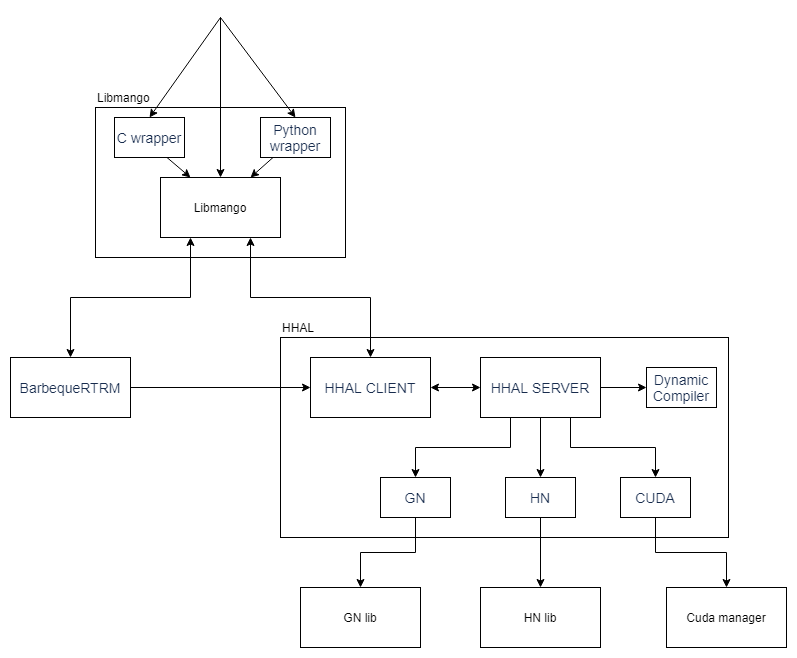
\includegraphics[scale=0.5]{img/architecture.png}

\section{Core elements}
Throughout the multiple MANGO modules, there are a few core elements often present in each module. These are the components necessary to specify and control an user application and its execution. Although their names may vary from module to module, here they are defined as Kernel, Memory Buffer, Event and Task graph.

\subsection{Kernel}
In computing, a compute kernel is a routine compiled for high throughput accelerators (such as graphics processing units (GPUs), digital signal processors (DSPs) or field-programmable gate arrays (FPGAs)), separate from but used by a main program (typically running on a central processing unit). \cite{kernel_wikipedia}

The MANGO system manages user defined Kernels and their execution. For a particular Kernel, multiple sources (accelerator specific implementations of the kernel) can be specified. The architectures for which an implementation is available are considered in the kernel-accelerator assignation process by the resource manager. 

As any computer program, a kernel must have the capability of interacting with the outside world in order to perform significant work. This is achieved through the support of kernel arguments.

%TODO styling
Three types of kernel arguments are supported: 
\begin{itemize}
    \item Scalar Argument: A scalar value. For example, an integer.
    \item Buffer Argument: A pointer to a Memory Buffer.
    \item Event Argument: A pointer to an Event data type.
\end{itemize}

\subsection{Memory Buffer}
%TODO better diagram
\begin{figure}[ht]
    \centering
    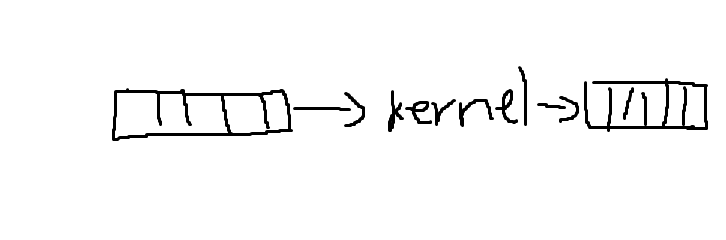
\includegraphics[width=\textwidth]{img/kernel_buffer.png}
    \captionsetup{justification=centering}
    \caption{Input and Output Buffers}
    \label{fig:in_out_buffers}
\end{figure}

In computer science, a data buffer (or just buffer) is a region of a physical memory storage used to temporarily store data while it is being moved from one place to another. \cite{buffer_wikipedia}

Kernels read from Input Buffers and write to Output Buffers for inter-kernel and host-kernel data transfering.

A Memory Buffer is defined by the user and allocated by MANGO at the target architectures, where a Kernel that makes use of said Buffer (as either input or output) is assigned.

\subsection{Event}

An event is a data structure utilized for communication and synchronization of different parts of the system.

User defined events can be accessed by Kernels through Event Arguments, providing the user with the necessary tools for the implementation of host-kernel or inter-kernel synchronization.

By default, MANGO utilizes kernel termination events for both internal and host synchronization.

\subsection{Task Graph}

The Task Graph gives a global picture of the application's behaviour and represents data and control dependencies between Kernels, Memory Buffers and Events. The Task Graph provides the resource manager with the information needed to generate the best feasible resource allocation for the requested QoS. \cite{mango_exploring_manycore_architectures} % TODO: define as QoS - Tomas


\section{Libmango}
Libmango is the front-facing module of the MANGO system, hence providing the system's API for user interaction with the underlying components, and acting as an abstraction layer between user defined models and module specific requirements.

The goal of the Libmango module is to allow software stack developers to easily map high-level programming models on the range of supported accelerators. Through the communication with the BarbecueRTRM and HHAL modules, user models are automatically mapped to the supported accelerators in a transparent manner, removing integration complexity from the user's hands.

The Libmango API allows developers to indicate to the runtime the components of their application, namely kernels, memory buffers and events. These are grouped in a task graph that represents the dependencies among the multiple components. 

Libmango is implemented in the C++ programming language, so its native usage is through the C++ API. However, a set of wrappers for other languages are provided, namely the C and Python API wrappers.

\subsection{Context}
The Context is the main class in the Libmango module, it holds the state information of the host side runtime for a single application, and its created by the user at the beginning of their interaction, with an application name and a recipe file needed by BarbecueRTRM for the resource allocation. Every subsequent component (kernels, buffers, events and task graph) has to be registered in the Context in order to be considered part of the application. % TODO: explain that the recipe contains resource allocation information, but is explained further in a following section - Tomas

Once the application is specified, the task graph information is sent to the BarbecueRTRM for the resource allocation. After a successful resource allocation, the application is now ready to run.

\subsection{Kernel management} \label{Libmango:KernelManagement}
Libmango exposes functionalities and data structures that can be used to represent and manipulate kernels.

Kernels are identified by an user-provided integer. For a single kernel, multiple implementations can be specified, each one targeting a different supported accelerator and thus provided in their respective architecture's requirements - a kernel implementation targeting an Nvidia GPGPU would require a CUDA implementation.
Kernel versions (implementations) are stored either in memory or in external files. According to the targeted architecture, multiple source types are supported. The kernel source can be a pre-compiled binary file or code in accelerator-supported language, provided via a string stored in memory or a source file, to be dynamically compiled if required.
The resource manager will rely on the available options in the assignation of kernels to accelerators.

Kernels can be manually started by the developer once the resource allocation is successfully completed.

Libmango supports three types of Kernel arguments: Scalar arguments, Buffer arguments and Event arguments.
These essentially act as wrappers of the HHAL kernel arguments.

\subsubsection{Scalar argument}
A Scalar argument consists of a scalar value. The types supported by Libmango are signed and unsigned integers of sizes 8, 16 and 32 bits, as well as long and float values. % TODO: long is just a 64 or 32 bit integer depending on the architecture. I would just remove this and add 64 bit integers.  Also we are replicating this in the HHAL section, should be unified somewhere. - Tomas
When a Scalar argument is created, the provided value is copied and stored in memory, and later sent to the HHAL module when their respective kernel is ran. 

\subsubsection{Buffer argument}
A Buffer argument consists of a Buffer integer identifier. The corresponding memory pointer in the accelerator's memory space is passed as an argument to the Kernel at execution time.

%TODO better explain how the kernel function receives the event argument depending on the architecture
\subsubsection{Event argument}
An Event argument consists of an Event integer identifier. The corresponding Event is passed as an argument to the Kernel at execution time.


\subsection{Buffer management}
Libmango exposes functionalities and data structures that can be used to represent and manipulate Memory Buffers. Buffers are the main data communication instruments between the host and the executing Kernels. 

A Buffer is identified by an user-provided integer. It consists of a pointer to a memory location where the Memory Buffer starts, and its size in bytes. 
For creating a Buffer, the user needs to register it to the application's Context. A Buffer is automatically allocated in the same accelerator where the Kernel that writes to, or reads from it, is assigned to by the resource manager.
Once successfully allocated, Libmango permits the writing of the Buffer with host-side data, as well as reading from the Buffer into host memory.


\subsection{Event management}
To provide developers with synchronization capabilities, Libmango exposes Event functionalities.

An Event is identified by an integer generated by Libmango. Events are synchronization data structures with an internal value utilized to indicate the different stages in the process, or in the case of user-defined Events, any denotation the user gives it.

Libmango lets the user define their own Events. These can be passed as arguments to the Kernels (if the target architecture supports them), which allows for user-defined inter-Kernel or host-Kernel synchronization.

By default, Libmango utilizes Events for Kernel termination synchronization. For every registered Kernel, Libmango automatically generates a Kernel-termination Event, which can also be accessed by the developers for waiting until a started Kernel finishes.

\subsection{API Wrappers}
As the core implementation of Libmango is in the C++ programming language, a set of wrappers are provided to complement the C++ API and allow developers to make use of the MANGO system using their programming language of choice.

Besides the native C++ API, Libmango currently exposes C and Python API wrappers.

\subsubsection{C API Wrapper}
% TODO: this doesn't say much. The most important part of the C API is hiding the object oriented C++ and smart pointers. Also I'm pretty sure using uint32_t addressing is wrong, but a problem of the GN library. - Tomas

The C language API is a wrapper around the C++ API that is provided both for compatibility with C code and for compatibility with the early version of MANGO, which was developed in C.

All the data types in the function prototypes have been made opaque using specific typedef types. This hides to the application some specific types of the machine, such as the size of the memory addresses. In the current MANGO implementation, the used types are mostly uint32\_t, due to the addressing size that is of 32-bit.

The API is divided in 8 groups: initialization and shutdown, kernel loading, task graph definition, task graph registration, resource allocation, kernel launching, synchronization primitives, and data transfer. \cite{mango_exploring_manycore_architectures}

\subsubsection{Python API Wrapper}

The Python wrapper aims at expanding MANGO accessibility onto scripting programming languages. Due to the nature of the MANGO system, scripting languages are a perfect fit, as the computation-heavy part of the user application are often the kernels executed in the available accelerators.

Python's popularity as a programming/scripting language made it an ideal candidate to enable a great number of developers access to the MANGO platform. As observed in figure \ref{fig:redmonk-ranks}, Python was the second most popular programming language in the RedMonk's Programming Language Rankings \cite{redmonks_rankings}, only falling behind JavaScript.

%TODO fixed location for now, check later to see what to do
% Just changing it to [ht] should be fine, depending on what we rewrite it will probably shift positions. - Tomas. 
\begin{figure}[H]
    \centering
    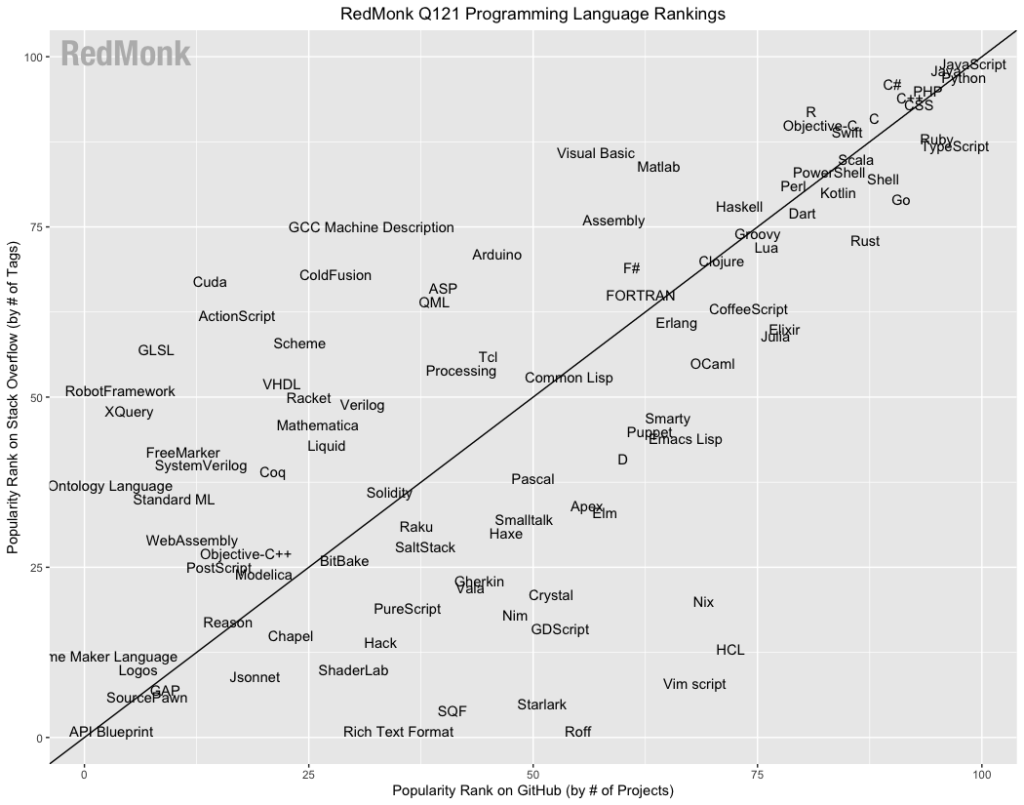
\includegraphics[width=\textwidth]{img/redmonk-ranks.png}
    \captionsetup{justification=centering}
    \caption{RedMonk's January 2021 Programming Language Rankings}
    \label{fig:redmonk-ranks}
\end{figure}

The Python API wrapper is implemented using Cython, with support for Python 3. Cython is an optimising static compiler that allows writing Python code that calls back and forth from and to C or C++ code natively at any point \cite{cython}.
For the API user, Cython usage is completely transparent and not a requirement, so their code can be purely written in Python. 

% TODO: where did the Event "ev" come from? Also we should choose the same notation for omitting stuff.
% Check the snippets in state of the art. - Tomas
\begin{lstlisting}[style=PythonStyle, caption=Python API Example snippet]
# Omitted: Register kernel(k), buffers(b1,b2,b3) and build task graph(tg)
with ctx.resource_allocation(tg):
    arg1 = BufferArg(b1)
    arg2 = BufferArg(b2)
    arg3 = BufferArg(b3)
    arg4 = ScalarArg(size, ScalarType.INT)

    args = KernelArguments(k, arg1, arg2, arg3, arg4)

    b1.write(A.tobytes())
    b2.write(B.tobytes())

    end_event = ctx.start_kernel(k, args)

    ev.wait()
    b3.read(C)

    end_event.wait()
# Omitted: Check results
\end{lstlisting}


\subsection{Sample Application}

In this section we will go over a sample to showcase and explain the Libmango C++ API usage. The sample application consists on the computation of a SAXPY operation (z = ax + y) over two trivially pre-initialized arrays: x and y. 

\begin{lstlisting}[style=CStyle, caption=saxpy.cu]
extern "C" __global__ 
void saxpy(float a, float *x, float *y, float *out, int n) {
  size_t tid = blockIdx.x * blockDim.x + threadIdx.x;
  if (tid < n) {
    out[tid] = a * x[tid] + y[tid];
  }
}
\end{lstlisting}

The target architecture of the sample is CUDA, hence a precompiled binary of the shown CUDA kernel that performs the SAXPY operation is used.

% TODO: I would put all the sample in one listing, ommitting unnecessary stuff like includes, stdouts and buffer initialization. That way it can be compared more closely with the snippets in state of the art. - Tomas
\begin{lstlisting}[style=CStyle, caption=Sample - Includes]
#include <cstddef>
#include <iostream>
#include <memory>

#include <host/context.h>
#include <host/logger.h>
\end{lstlisting}

First we set up the sample with the necessary includes. Regarding Libmango, \textbf{context.h} is the required header that exposes the C++ API. \textbf{logger.h} is also included to access the Libmango logger.

\begin{lstlisting}[style=CStyle, caption=Sample - Definitions]
#define KERNEL 1
#define B1 1
#define B2 2
#define B3 3

// saxpy function matching the CUDA kernel, used to check the results
void saxpy(float a, float *x, float *y, float *o, float n) {
    for (size_t i = 0; i < n; ++i) {
        o[i] = a * x[i] + y[i];
    }
}
\end{lstlisting}

We now define the kernel and buffers integer identifiers, as well as a \textbf{saxpy} function that matches the \textbf{saxpy.cu} kernel computation, we will use it to check the obtained results.

\begin{lstlisting}[style=CStyle, caption=Sample - Initialization]
int main(int argc, char const *argv[])
{
    // Initialization
    mango::mango_init_logger();
    auto mango_rt = mango::Context("cuda_simple", "test_manga_cuda");

    int n = 4096;
    size_t buffer_size = n * sizeof(float);
    float a = 2.5f;
    float *x = new float[n], *y = new float[n], *o = new float[n];

    for (size_t i = 0; i < n; ++i) {
        x[i] = static_cast<float>(i);
        y[i] = static_cast<float>(i * 2);
    }
\end{lstlisting}

%TODO we mention the recipe file here, it will probably get explained under BarbecueRTRM later, so link to that and clarify
At the beginning of the \textbf{main} function, we initialize the logger, and the application's \textbf{Context} is created. For the initialization of the Context, an application name is required: "cuda\_simple", as well as a recipe file name for the BarbecueRTRM resource allocation: "test\_manga\_cuda".

Then, the three buffers we need for the operation are declared. \textbf{x} and \textbf{y} are the input buffers, so they are initialized with known values. \textbf{o} is the output buffer where we will store the results, so there is no need to initialize its data.

\begin{lstlisting}[style=CStyle, caption=Sample - Kernel loading]
    char kernel_path[] = "/opt/mango/usr/local/share/cuda_simple/saxpy";
    auto kf = std::make_shared<mango::KernelFunction>();
    kf->load(kernel_path, mango::UnitType::Nvidia, mango::FileType::BINARY);
\end{lstlisting}

To load the saxpy kernel binary file, we create a \textbf{KernelFunction} object, and then load the kernel through the \textbf{load()} function, specifying the target architecture and file type.

\begin{lstlisting}[style=CStyle, caption=Sample - TaskGraph registration and resource allocation]
    // Registration of task graph
    auto k  = mango_rt.register_kernel(KERNEL, kf, {B1, B2}, {B3});

    auto b1 = mango_rt.register_buffer(B1, buffer_size, {}, {KERNEL});
    auto b2 = mango_rt.register_buffer(B2, buffer_size, {}, {KERNEL});
    auto b3 = mango_rt.register_buffer(B3, buffer_size, {KERNEL}, {});

    auto tg = mango::TaskGraph({k}, {b1, b2, b3});

    // Resource Allocation
    mango_rt.resource_allocation(tg);
\end{lstlisting}

In order to realize the resource allocation, we first need to register the elements in the Context and create the \textbf{TaskGraph}.
The kernel is registered in the Libmango Context by providing its id, kernel function and input and ouput buffers.
The buffers are registered by providing their ids, size, kernels where they act as input and kernels where they act as output.

Finally, the \textbf{TaskGraph} is created with the previously registered elements and the resource allocation is performed over the specified TaskGraph.

\begin{lstlisting}[style=CStyle, caption=Sample - Arguments set up]
    auto argX = mango::BufferArg(b1);
    auto argY = mango::BufferArg(b2);
    auto argO = mango::BufferArg(b3);
    auto argA = mango::ScalarArg<float>(a);
    auto argN = mango::ScalarArg<int>(n);

    auto argsKERNEL = mango::KernelArguments({argA, argX, argY, argO, argN}, k);
\end{lstlisting}

The \textbf{saxpy} kernel receives five arguments, two scalars and three buffers. A \textbf{BufferArg} is created for each buffer argument, and two \textbf{ScalarArg} are created with their respective types (float and int) for each of the scalar arguments.

A \textbf{KernelArguments} object groups the arguments to be passed to a given kernel in the stated order.

\begin{lstlisting}[style=CStyle, caption=Sample - Writing buffers]
    std::cout << "Sample host: Writing to buffer 1..." << std::endl;
    b1->write(x, buffer_size);

    std::cout << "Sample host: Writing to buffer 2..." << std::endl;
    b2->write(y, buffer_size);
\end{lstlisting}

Before launching the kernel, we need to write the data from the host buffers onto the registered buffers that where allocated at the target accelerators in the resource allocation. To write to a buffer, we use the \textbf{write()} function of the \textbf{Buffer} objects that were returned from the Context registration.
    
\begin{lstlisting}[style=CStyle, caption=Sample - Kernel launch]
    std::cout << "Sample host: Starting kernel..." << std::endl;
    auto e = mango_rt.start_kernel(k, argsKERNEL);

    std::cout << "Sample host: Waiting for kernel completion..." << std::endl;
    e->wait();
\end{lstlisting}

We are now ready to execute the kernel. The \textbf{start\_kernel()} function takes the kernel and its arguments and returns a kernel termination \textbf{Event}. By calling the event's \textbf{wait()} function, the host execution is blocked until the kernel's termination is notified.

\begin{lstlisting}[style=CStyle, caption=Sample - Checking results]
    b3->read(o, buffer_size);

    float *expected = new float[n];
    saxpy(a, x, y, expected, n);

    bool correct = true;
    for (int i = 0; i < n; ++i) {
        if (o[i] != expected[i]) {
            std::cout << "Sample host: Error!\n" << std::endl;
            correct = false;
            break;
        }
    }
    if(correct) {
        std::cout << "Sample host: SAXPY correctly performed!" << std::endl;
    }
\end{lstlisting}

Once the kernel terminated, we can read the results from the output buffer \textbf{b3}. By using the buffer's \textbf{read()} function, we can read the data from the accelerator's memory into the \textbf{o} host buffer.

We use the \textbf{saxpy} function defined at the beginning of the sample to check the correctness of the results.

\begin{lstlisting}[style=CStyle, caption=Sample - Teardown]
    mango_rt.resource_deallocation(tg);
    delete[] x;
    delete[] y;
    delete[] o;
    delete[] expected;

    return 0;
}
\end{lstlisting}

Before returning, we perform the resource deallocation of the TaskGraph, and free the host buffers.

\section{BarbecueRTRM}

The MANGO architecture is based on the idea of building energy efficient HPC (High Performance Computing) systems. In heterogeneous architectures, the resource management problem is especially complex due to the difficulty of scheduling tasks over multiple architectures with different instruction sets and requirements.

A resource manager performs the tasks scheduling and assignation of resources to the available accelerators, according to the application's objective, like the minimization of power consumption or the minimization of execution time. \cite{mango_exploring_manycore_architectures}

The framework used for resource management in the MANGO system is the Barbeque Run-Time Resource Manager (BarbecueRTRM). 
The BarbequeRTRM is a modular and extensible run-time resource manager, to manage the allocation of computing resources (e.g, CPU, GPU, memory, HW accelerators, etc…) to multiple concurrent applications. Its modular design allows the developers to add custom resource allocation policies, according to specific use-cases and target platforms. \cite{barbecue_1}\cite{barbecue_2} % TODO: I think there is something missing in the first sentence, also no "..." pls. - Tomas

\subsection{Resource Manager Architecture}

\begin{figure}[ht]
    \centering
    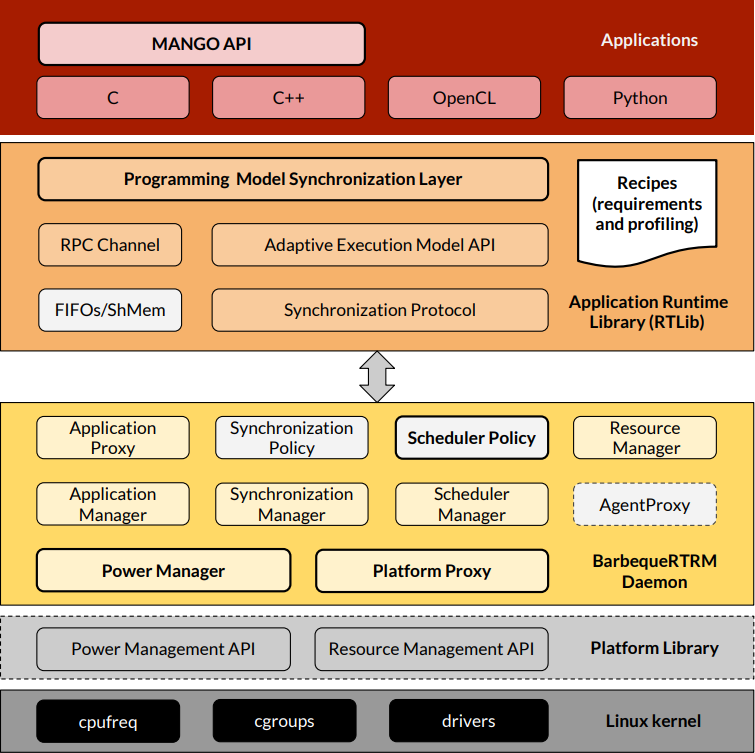
\includegraphics[width=\textwidth]{img/barbecue-arch.png}
    \captionsetup{justification=centering}
    \caption{Overview of the BarbequeRTRM}
    \label{fig:barbecue-arch}
\end{figure}

In figure \ref{fig:barbecue-arch}, we can see an overview of the BarbecueRTRM framework. The interfacing with the rest of the MANGO system happens at application level, specifically Libmango natively communicates with the Application Runtime Library (RTLib) implemented in C++, which in turns acts as a client of the BarbecueRTRM Daemon running in the host system.

The Programming Model Synchronization Layer in the RTLib facilitates MANGO integration with the BarbecueRTRM by working as an abstraction layer that supports the MANGO programming model for a BarbecueRTRM managed application.
The Libmango-BarbecueRTRM interaction happens through an \textbf{Application Controller}, which is created when a Libmango \textbf{Context} is initialized.

The daemon and applications communicate through a Remote Procedure Call (RPC) based protocol. Data are mainly exchanged by using named pipes; a general one for the messages coming from the application to the resource manager, plus one pipe per application for application management purposes. A further communication channel, based on shared memory, has been introduced in MANGO to enable an efficient transfer of complex data structures, like for example the task-graph representations of the applications. 

Regarding hardware support, suitable system interfaces for accessing low-level mechanisms are required. The two components that create an abstraction layer on top of the platform and resource specific interfaces are the \textbf{Platform Proxy} and the \textbf{Power Manager}. Examples of such interfaces are the Linux frameworks cgroup and cpufreq, used to bound the amount of CPU time, memory and number of CPU cores assigned to an application, as well as managing the clock frequency of cores.
There are, of course, resources out of the Linux operating system control, in these cases platform-specific libraries are used, for example the NVIDIA Management Library (NVML) \cite{nvml} is utilized for controlling and obtaining runtime data of NVIDIA GPUs. \cite{mango_exploring_manycore_architectures}

The \textbf{Platform Proxy} also performs the resource assignation. This is done through functions exposed by the \textbf{HHAL API}, for which a specific Platform Proxy must have an HHAL Client.

- scheduler policy


\subsection{Integration}

As previously stated, The Libmango-BarbecueRTRM communication is done through an Application Controller, which is created when a Libmango Context is initialized.

%TODO update names in the diagram
\begin{figure}[ht]
    \centering
    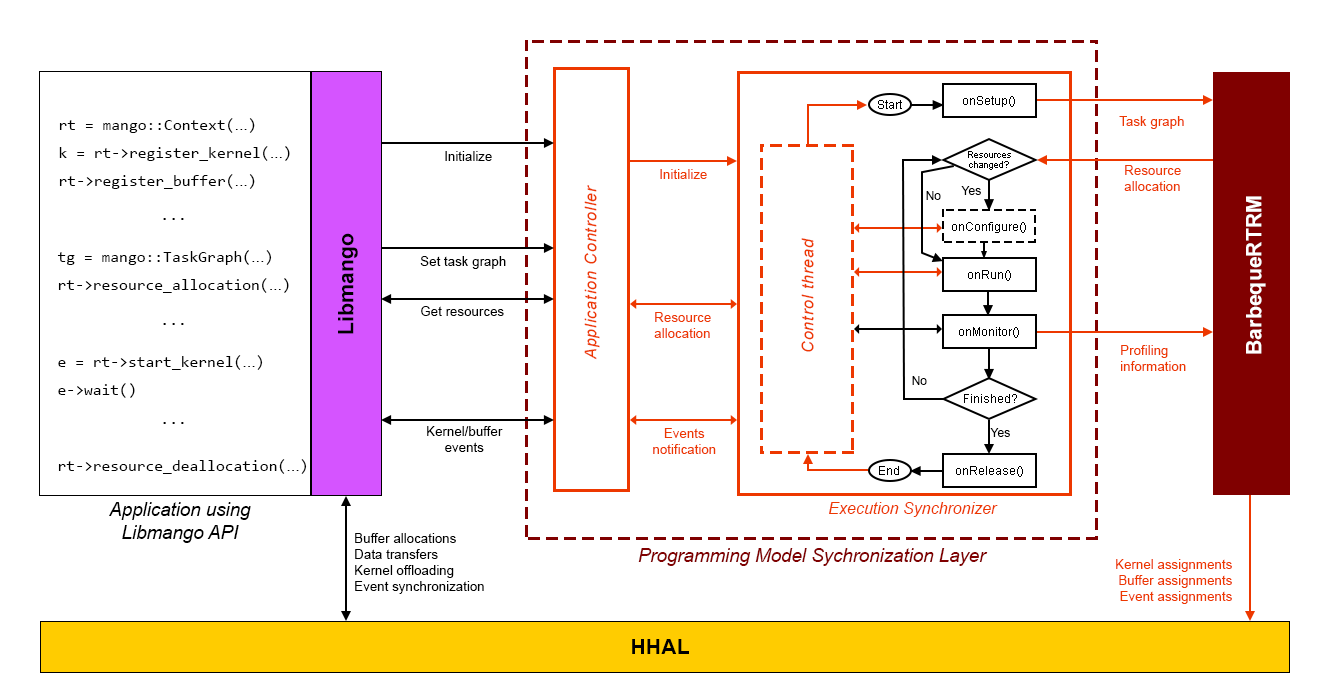
\includegraphics[width=\textwidth]{img/barbeque-flow.png}
    \captionsetup{justification=centering}
    \caption{Flow between BarbequeRTRM and the MANGO system}
    \label{fig:barbecue-flow}
\end{figure}


- recipes



\section{HHAL}

%TODO add a graph showing hhal: client, server, api, managers, dycomp

The Heterogeneous Hardware Abstraction Layer (HHAL) is the module of the MANGO system that takes care of the communication with the multiple accelerator libraries.
As such, HHAL abstracts accelerator specific information in a manner that allows the resource manager to fully exploit architecture specific features, while freeing libmango from the inherent complexity of handling multiple architectures.

% TODO a daemon is mentioned previously in BBQUE, also maybe it is not necessary to include a definition.
% We will probably have to add a definitions section / glossary for any definitions. - Tomas
Due to the fact that multiple modules running as independent processes need to make use of the Heterogeneous Hardware Abstraction Layer, HHAL works in a client-server manner. The server is run as a daemon, or background process \cite{daemon_wikipedia}, and the client is used by other modules to interact with it. In this way, both BarbecueRTRM and Libmango can make use of a common instance of the HHAL module.

HHAL exposes an architecture-agnostic API with the necessary functionalities to permit the managing of kernels, buffers and events on any of the supported architectures. The module is structured as a front-facing API and a set of architecture specific managers that implement the API functionalities for their specific architecture.

\subsection{Abstracting architecture-specific information}

Due to the fact that a single API is utilized for interacting with every supported architecture, underlying architecture managers require a mechanism that allows the description of architecture specific information by external modules, specifically the resource manager.

For each resource, there is a base structure that contains the minimal information required by the front-facing API, namely the resource's identification integer. 

\begin{lstlisting}[style=CStyle, caption=HHAL API - Base structures]
typedef struct hhal_kernel_t {
    int id;
} hhal_kernel;

typedef struct hhal_buffer_t {
    int id;
} hhal_buffer;

typedef struct hhal_event_t {
    int id;
} hhal_event;
\end{lstlisting}

Architecture managers can expand these base structures to add architecture specific information that they may require. For example, the following are the structures used by the Nvidia Manager.

\begin{lstlisting}[style=CStyle, label={HHAL:NvidiaStructs}, caption=HHAL Nvidia Manager - Extended structures]
typedef struct nvidia_kernel_t {
    int id;
    int gpu_id;
    int mem_id;
    uint32_t grid_dim_x;
    uint32_t grid_dim_y;
    uint32_t grid_dim_z;
    uint32_t block_dim_x;
    uint32_t block_dim_y;
    uint32_t block_dim_z;
    int termination_event;
} nvidia_kernel;

typedef struct nvidia_buffer_t {
    int id;
    int gpu_id;
    int mem_id;
    size_t size;
    std::vector<int> kernels_in;
    std::vector<int> kernels_out;
} nvidia_buffer;

typedef struct nvidia_event_t {
    int id;
} nvidia_event;
\end{lstlisting}

The general API essentially acts as a dispatcher, and passes the casted structure pointer when calling the corresponding manager function. 

The following code snippet is for example purposes and not part of the final implementation.

\begin{lstlisting}[style=CStyle, caption=HHAL API Example - Dispatching architecture-specific structures]
void HHAL::example_function(Unit unit, hhal_kernel *info) {
    switch (unit) {
        case Unit::GN:
            GN_MANAGER.example_function((gn_kernel *) info);
            break;
        case Unit::NVIDIA:
            NVIDIA_MANAGER.example_function((nvidia_kernel *)info);
            break;
    }
}
\end{lstlisting}

%TODO better diagram
\begin{figure}[ht]
    \centering
    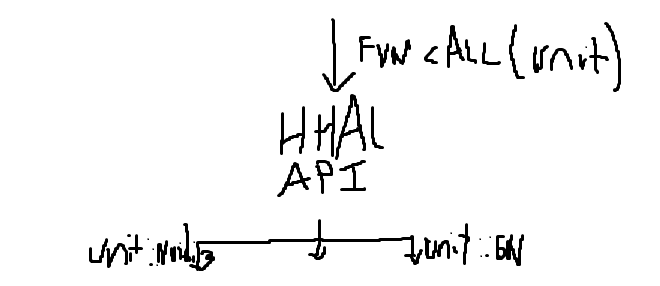
\includegraphics[width=\textwidth]{img/hhal_dispatcher.png}
    \captionsetup{justification=centering}
    \caption{HHAL API dispatching flow}
    \label{fig:hhal_dispatcher}
\end{figure}

\subsection{HHAL API}

The API exposed by HHAL provides a set of functionalities for managing resources. Here we explain in detail each functionality and how they relate to each component of the user's application: kernels, buffers and events.

\subsubsection{Resource Assignation}

Each resource composing the overall user application is assigned to an architecture by the resource manager. The resource assignation takes place before the allocation in its assigned target accelerator, and its the step in which the resource's information is made known to HHAL.

In the assignation process, an identification integer is provided for the resource being assigned. This same id is utilized in successive operations to map a resource with the information provided at assignation time.

To assign a resource, a supported unit where the resource is to be assigned is provided in the function call. Further usage of the resource will automatically be handled by the corresponding architecture manager.

\begin{lstlisting}[style=CStyle, caption=HHAL API - Assign functions]
    HHALExitCode assign_kernel(Unit unit, hhal_kernel *info);
    HHALExitCode assign_buffer(Unit unit, hhal_buffer *info);
    HHALExitCode assign_event (Unit unit, hhal_event *info);

    HHALExitCode deassign_kernel(int kernel_id);
    HHALExitCode deassign_buffer(int buffer_id);
    HHALExitCode deassign_event(int event_id);
\end{lstlisting}

% TODO: HHAL Module -> HHAL Runtime? - Tomas
Once a resource is no longer required by the application, it may be deassigned and thus removed from the HHAL module.

\subsubsection{Resource Allocation}

Every assigned resource has to eventually be allocated in its target accelerator in order for their associated kernel/s to be able to run.

Both allocation and release (deallocation) function calls are simple, due to the fact that the required information regarding the resources is provided beforehand at assignation time. Thus, only the resource's identification integer is needed.

% TODO: Should group this like assignments to keep it consistent - Tomas
\begin{lstlisting}[style=CStyle, caption=HHAL API - Allocation functions]
    HHALExitCode allocate_kernel(int kernel_id);
    HHALExitCode release_kernel(int kernel_id);

    HHALExitCode allocate_memory(int buffer_id);
    HHALExitCode release_memory(int buffer_id);

    HHALExitCode allocate_event(int event_id);
    HHALExitCode release_event(int event_id);
\end{lstlisting}

The resource's target architecture manager is dispatched the allocation/deallocation action and it takes care of the accelerator specific requirements for allocating resources.

\subsubsection{Buffer Actions}

Memory Buffers that are allocated in an accelerator have to be capable of being written and read. The HHAL API provides write and read functions that take the buffer's id, a pointer to a source/destination buffer in the host memory space and the size of the buffer.

\begin{lstlisting}[style=CStyle, caption=HHAL API - Buffer actions]
    HHALExitCode write_to_memory(int buffer_id, const void *source, size_t size);
    HHALExitCode read_from_memory(int buffer_id, void *dest, size_t size);
\end{lstlisting}

Communication with the corresponding accelerator is handled by the architecture's manager.

\subsubsection{Event Actions}
% TODO: maybe we should change the code to refer to events, or just change the names here. "sync_register" adds unnecessary confusion. - Tomas
Events that are allocated in an accelerator require the capability of being written and read. The HHAL API provides a write function that takes the event's id and the data to write, and a read function that takes the event's id and a pointer to host memory where to read the data into.

\begin{lstlisting}[style=CStyle, caption=HHAL API - Event actions]
    HHALExitCode write_sync_register(int event_id, uint32_t data);
    HHALExitCode read_sync_register(int event_id, uint32_t *data);
\end{lstlisting}

Once again, accelerator specifics are handled by the architecture's manager. In some cases (like Nvidia), events are handled entirely on the Nvidia Manager, as the Nvidia Architecture Node does not provide events support.

\subsubsection{Kernel Actions} \label{HHAL:KernelActions}
% TODO: ran -> run. - Tomas
Before a Kernel is ran, its source first has to be written into the accelerator's memory. The HHAL API provides a kernel write function that takes the kernel's id and a map of unit to sources, out of which the previously assigned unit's source is taken.

Multiple kernel's source types are supported by HHAL, this is further explained in the Dynamic Compiler \ref{HHAL:DynamicCompiler} subsection.

\begin{lstlisting}[style=CStyle, caption=HHAL API - Kernel actions]
    HHALExitCode kernel_write(int kernel_id, const std::map<Unit, hhal_kernel_source> &kernel_sources);
    HHALExitCode kernel_start(int kernel_id, const Arguments &arguments);
\end{lstlisting}

% TODO: ran -> run. - Tomas
After a Kernel is written and its dependencies are correctly set up, it can be ran, or "started" via the kernel start function. As kernels require argument support, this function not only takes the kernel's id but also an \textbf{Arguments} object which consists of a vector of kernel arguments.

Three types of arguments are supported by HHAL: Scalar arguments, Buffer arguments and Event arguments. These are the arguments wrapped by Libmango for the user to provide. \ref{Libmango:KernelManagement} 

Scalar arguments consist of a scalar value belonging to one of the supported types. These are signed and unsigned integers of sizes 8, 16, 32 bits as well as long and float values. % TODO: long is just a 64 or 32 bit integer depending on the architecture. I would just remove this and add 64 bit integers, also doubles.

The Buffer and Event arguments consist of the respective's Buffer or Event id, which is used to pass the corresponding structure information to the Kernel.

\subsection{Dynamic Compiler} \label{HHAL:DynamicCompiler}

% TODO: an user -> a user. - Tomas
In previous implementations of the MANGO system, an user provided Kernel had to be pre-compiled into a binary file (or the format required by the target accelerator) before its utilization in the MANGO system. Despite the optimalilty of this process, it puts limits on the agile and iterative nature of the development of software solutions.

% TODO: Pre-compilation wouldn't really help with performance if we take into account that the binary will be cached and the user could provide custom flags (although I think it's not implemented yet). - Tomas
Giving developers the ability to work directly with kernel source code greatly facilitates the development process. Ideally, once a solution is in place, kernels would be pre-compiled for optimal perfomance.

% TODO: Wrong paragraph order? - Tomas
The Dynamic Compiler included in the HHAL module offers the functionality of "dynamic" compilation of kernels. That is, the developer provides a kernel's source code to be compiled as required before being written into its target accelerator's memory.

\subsubsection{Usage and Implementation}

As previously mentioned, HHAL supports multiple types of kernel sources: 

\begin{lstlisting}[style=CStyle, caption=HHAL API - Kernel source types]
enum class source_type {
    BINARY,
    SOURCE,
    STRING
};
\end{lstlisting}

The \textbf{BINARY} type is for pre-compiled kernels in binary format. While \textbf{SOURCE} and \textbf{STRING} refer to source code in a file or in a string in memory respectively.

The Dynamic Compiler is automatically used by HHAL when either a SOURCE or a STRING source type is provided in the kernel write function call. \ref{HHAL:KernelActions}

The usage of the Dynamic Compiler is simple, requiring only the instantiation of a \textbf{Compiler} object, and a single \textbf{get\_binary()} function call to obtain a kernel's binary from its source.

\begin{lstlisting}[style=CStyle, caption=HHAL Dynamic Compiler - Compiler class]
class Compiler {
    public:
        Compiler();
        const std::string get_binary(const std::string source, hhal::Unit arch);

        [...]
};
\end{lstlisting}

Internally, the Dynamic Compiler has a set of alternatives to work with, depending on its configuration and the target architecture of a specific source.

For kernel sources belonging to the C family, the Clang frontend for the LLVM project \cite{clang_llvm} is utilized if enabled and installed in the user's machine.

Otherwise, compilation is done through system calls as specified in the configuration, utilizing a compiler tool installed in the user's machine.

In the case of CUDA kernels (targeting Nvidia accelerators), the CUDA Compiler tool \ref{Nvidia:CudaCompiler} from the Nvidia Architecture Node is utilized for compilation. This tool exploits the CUDA runtime compilation library NVRTC to compile CUDA kernels into a ptx format as required by the Nvidia Architecture Node.

\subsubsection{Configuration} \label{HHAL:DynamicCompilerConfiguration}

On initialization, the Dynamic Compiler reads a configuration file located in its installation directory. Through this configuration, the user can specify the tools to utilize for the compilation process.

\begin{lstlisting}[style=CStyle, caption=HHAL Dynamic Compiler - Configuration example]
[compiler]
expiration=86400

[GN]
libclang=false
path=cc

// Syntax
[ARCHITECTURE_NAME]
libclang=true_or_false
path=path_to_compiler
\end{lstlisting}

In the previous configuration example, under \textbf{[compiler]}, the \textbf{expiration} time for compilation related kernel files is specified in seconds, this parameter is further explained in the Caching subsection \ref{HHAL:DynamicCompilerBinaryCaching}.

Then, for each supported architecture (\textbf{[ARCHITECTURE\_NAME]}), two parameters can be specified:
\begin{itemize}
    \item \textbf{libclang:} Whether the Clang compiler should be used when compiling kernels for this architecture.
    \item \textbf{path:} The path to a compiler tool installed in the user's machine to be used when compiling kernels for this architecture. Also works as a fallback option if libclang is not available in the system.
\end{itemize}

\subsubsection{Caching} \label{HHAL:DynamicCompilerBinaryCaching}

The Dynamic Compiler implements a caching mechanism to avoid the re-compilation of previously used kernels, exchanging disk space for processing time.

When a kernel is compiled, the compilation output is saved into a file under the caching directory specified at installation. Each time a kernel is sent to the Dynamic Compiler for compilation, an internal check is performed to see whether the source file has already been compiled. This is done by checking if there is a compiled kernel file with the same name as the source file, and if the source file has been modified since.

\begin{lstlisting}[style=CStyle, caption=HHAL Dynamic Compiler - Save kernel string to file]
const std::string save_to_file(const std::string kernel_string);
\end{lstlisting}

If the kernel was loaded as a memory string, HHAL first calls the \textbf{save\_to\_file()} utility function, provided by the Dynamic Compiler, which saves the kernel string as a source file, and then uses this file for compilation. The saved source file is named with the hash of the input string, which allows for fast checking if a kernel source has already been saved.

To prevent the problem of ever-growing disk space usage, every time a kernel is sent for compilation, the Dynamic Compiler runs a procedure to delete unused (expired) files from the caching directory. The \textbf{expiration} time can be specified in the Dynamic Compiler configuration file \ref{HHAL:DynamicCompilerConfiguration}, defaulting to three days.

\subsubsection{Kernel entry generation}

For Kernels that fall under the GN architecture group, an entry point (main function) receiving the kernel's arguments as string values is required, since kernels are executed through a system call.

The Dynamic Compiler is capable of automatically generating the GN entry point, given that the user annotates the source kernel code accordingly, like in the following sample.

\begin{lstlisting}[style=CStyle, caption=HHAL Dynamic Compiler - Kernel source annotation sample]
#include "dev/mango_hn.h"
#include "dev/debug.h"
#include <stdlib.h>

#pragma mango_gen_entrypoint

#pragma mango_kernel
void kernel_function(int a, float *x, float *y, float *out, int n) {
    for (int i=0; i<n; i++) {
	    out[i] = a * x[i] + y[i];
    }
}
\end{lstlisting}

Two pragmas are required for the entry point generation. 

The first \textbf{\#pragma mango\_gen\_entrypoint} indicates that the entry point is to be generated. The second, \textbf{\#pragma mango\_kernel} must be placed a line before the function to be called by the generated entry point, as its arguments are the ones received by the main function.

%TODO include result of entrypoint generation here
<RESULT OF ENTRYPOINT GENERATION EXAMPLE HERE>

\subsection{Manager example: NVIDIA Manager}

HHAL was developed from the ground up with the goal of facilitating its extension via the addition of support for new architectures.

Each new architecture requires a manager that implements the HHAL API function calls for that architecture, acting as a bridge between the MANGO system and the particular target accelerator's library.

Modifications to the existing HHAL code resolve to the addition of the new architecture type and calls to the manager when dispatching the multiple API actions.

In this section, we will go over the Nvidia Manager to exemplify the implementation of an HHAL Manager. The Nvidia Manager communicates with the Nvidia Architecture Node \ref{NvidiaArchitectureNode}, referenced in code as \textbf{CudaApi}, which is the library implemented for launching kernels in Nvidia GPUs.

\begin{lstlisting}[style=CStyle, caption=HHAL Nvidia Manager - Manager Class]
class NvidiaManager {
    public:
        NvidiaManagerExitCode assign_kernel(nvidia_kernel *info);
        NvidiaManagerExitCode assign_buffer(nvidia_buffer *info);
        NvidiaManagerExitCode assign_event(nvidia_event *info);

        NvidiaManagerExitCode deassign_kernel(int kernel_id);
        NvidiaManagerExitCode deassign_buffer(int buffer_id);
        NvidiaManagerExitCode deassign_event(int event_id);

        NvidiaManagerExitCode kernel_write(int kernel_id, std::string image_path);
        NvidiaManagerExitCode kernel_start(int kernel_id, const Arguments &arguments);

        NvidiaManagerExitCode allocate_memory(int buffer_id);
        NvidiaManagerExitCode allocate_kernel(int kernel_id);
        NvidiaManagerExitCode allocate_event(int event_id);
        
        NvidiaManagerExitCode release_memory(int buffer_id);
        NvidiaManagerExitCode release_kernel(int kernel_id);
        NvidiaManagerExitCode release_event(int event_id);

        NvidiaManagerExitCode write_to_memory(int buffer_id, const void *source, size_t size);
        NvidiaManagerExitCode read_from_memory(int buffer_id, void *dest, size_t size);
        NvidiaManagerExitCode write_sync_register(int event_id, uint32_t data);
        NvidiaManagerExitCode read_sync_register(int event_id, uint32_t *data);
       
    private:
        void launch_kernel(int kernel_id, char *arg_array, int arg_count, char* scalar_allocations);

        std::map<int, nvidia_kernel> kernel_info;
        std::map<int, nvidia_buffer> buffer_info;
        std::map<int, nvidia_event> event_info;

        std::map<int, std::string> kernel_function_names;
        ThreadPool thread_pool;
        EventRegistry registry;
        CudaApi cuda_api;
};
\end{lstlisting}

The public function definitions mirror the HHAL API functions, which delegate the execution to the indicated manager. 

Observing the assignation functions, the received arguments are pointers to structures defined by the Nvidia Manager. As mentioned in the HHAL API section \ref{HHAL:NvidiaStructs}, these structures are extensions of the base structures used in the HHAL API, and they represent the three core elements of the MANGO system (kernels, buffers and events) with the addition of the information required by the Nvidia Architecture Node.

The Manager keeps track of the assigned elements in three different maps, one for each element, mapping the element's id to their respective extended data structure.

\begin{lstlisting}[style=CStyle, caption=HHAL Nvidia Manager - Kernel assignation]
NvidiaManagerExitCode NvidiaManager::assign_kernel(nvidia_kernel *info) 
{
    kernel_info[info->id] = *info;
    return NvidiaManagerExitCode::OK;
}
\end{lstlisting}

In assign/deassign functions, elements get added or removed from the maps respectively.

\subsubsection{Buffers}

Buffer allocation follows a simple procedure. The Nvidia Architecture Node takes a buffer id and size as parameters for the memory allocation call, so the manager just delegates the allocation given the information received at assignation time.

\begin{lstlisting}[style=CStyle, caption=HHAL Nvidia Manager - Kernel assignation]
NvidiaManagerExitCode NvidiaManager::allocate_memory(int buffer_id) {
    nvidia_buffer &info = buffer_info[buffer_id];
    CudaApiExitCode err = cuda_api.allocate_memory(info.mem_id, info.size);
    //error handling...
}
\end{lstlisting}

A similar course of action is followed in memory read and write operations, delegating their execution to the architecture library.

\subsubsection{Events}

Since the Nvidia Architecture Node does not support events, the Nvidia Manager handles them internally. This is carried out using an event registry, which implements the basic event functionalities.

\begin{lstlisting}[style=CStyle, caption=HHAL Nvidia Manager - Event registry]
class EventRegistry {
    public:
        EventRegistryExitCode add_event(int event_id);
        EventRegistryExitCode remove_event(int event_id);
        EventRegistryExitCode read_event(int event_id, uint32_t *data);
        EventRegistryExitCode write_event(int event_id, uint32_t data);
    private:
        std::mutex registers_mtx;
        std::map<int, uint32_t> registers;
};
\end{lstlisting}

Since event arguments are not supported for Nvidia kernels, only kernel termination events are handled.

\subsubsection{Kernels}

Aside from assignation and allocation, there are two main actions the manager must implement regarding kernels: write and start. 

\textbf{kernel\_write()} writes the kernel image in the accelerator's memory space. The Nvidia Manager also extracts the function name from the provided kernel, as it is required when on kernel launch.

\textbf{kernel\_start()} starts kernel execution in the target accelerator, with two relevant considerations: argument handling and non-blocking kernel launch.

The target architecture's library likely define their own kernel arguments, as is the case for the Nvidia Architecture Node, so they must be translated from the HHAL version into their Nvidia Architecture Node counterpart.

\begin{lstlisting}[style=CStyle, caption=HHAL Nvidia Manager - Kernel arguments translation]
NvidiaManagerExitCode NvidiaManager::kernel_start(int kernel_id, const Arguments &arguments) {
    //...
    char *current_arg = arg_array; //Base of arguments array to be sent to NAN
    for(auto &arg: args) {
        switch (arg.type) {
            case ArgumentType::BUFFER: {
                auto &b_info = buffer_info[arg.buffer.id];
                // Omitted: Check if buffer is an input buffer...
                auto *arg_x = (cuda_manager::BufferArg *) current_arg;
                *arg_x = {cuda_manager::BUFFER, b_info.id, is_in};
                current_arg += sizeof(cuda_manager::BufferArg);
                break;
            } 
            case ArgumentType::SCALAR: {
                hhal::scalar_arg scalar = arg.scalar;
                auto *arg_a = (cuda_manager::ScalarArg *) current_arg;
                // Omitted: Allocate scalar value locally so it's not deallocated until kernel terminates...
                *arg_a = {cuda_manager::SCALAR, (void *)allocated_scalar};
                current_arg += sizeof(cuda_manager::ScalarArg);
                break;
            }
            //...
}
\end{lstlisting}

Since the nature of MANGO requires kernel launching to be non-blocking, for each kernel start action a task executing the private \textbf{launch\_kernel()} procedure is added to an internal thread pool.

\begin{lstlisting}[style=CStyle, caption=HHAL Nvidia Manager - Kernel launch]
NvidiaManagerExitCode NvidiaManager::kernel_start(int kernel_id, const Arguments &arguments) {
    // Omitted: Argument translation...

    // Push launch_kernel task
    thread_pool.push_task(std::bind(&NvidiaManager::launch_kernel, this, kernel_id, arg_array, arg_count, scalar_allocations));

    return NvidiaManagerExitCode::OK;
}

void NvidiaManager::launch_kernel(int kernel_id, char *arg_array, int arg_count, char* scalar_allocations) {
    nvidia_kernel &info = kernel_info[kernel_id];

    CudaResourceArgs r_args = {info.gpu_id, 
                    {info.grid_dim_x, info.grid_dim_y, info.grid_dim_z, 
                    {info.block_dim_x, info.block_dim_y, info.block_dim_z}};

    auto &termination_event = event_info[info.termination_event];
    CudaApiExitCode err = cuda_api.launch_kernel(kernel_id, kernel_function_names[kernel_id].c_str(), r_args, arg_array, arg_count);

    // Omitted: Deallocation and error handling...

    // Notify kernel termination
    write_sync_register(termination_event.id, 1); 
}
\end{lstlisting}

Worker threads continuously execute pending tasks from the tasks queue managed by the thread pool. 
The \textbf{launch\_kernel()} function calls the Nvidia Architecture Node (blocking) procedure to execute the kernel and passes the necessary arguments.
Once the execution finishes, the kernel's termination event is notified.

\section{Nvidia Architecture Node} \label{NvidiaArchitectureNode}

- ptx format 
%https://docs.nvidia.com/cuda/inline-ptx-assembly/index.html#:~:text=The%20NVIDIA%C2%AE%20CUDA%C2%AE,the%20PTX%20ISA%20reference%20document.

\subsection{CUDA Compiler} \label{Nvidia:CudaCompiler}


\section{GN}

%TODO move somewhwere else
\section{HN}